\documentclass[a4paper]{article}
\newcounter{QuestionNumber}
\setcounter{QuestionNumber}{1}

\newcommand{\Q}{
\textbf{Question \theQuestionNumber)}
\stepcounter{QuestionNumber}
}
\usepackage{graphicx}
\usepackage{enumitem}
\usepackage[margin=1in]{geometry}
\usepackage{lipsum}
 \renewcommand{\familydefault}{\rmdefault}
\setlength{\parindent}{0pt}
\setlength{\parskip}{1em}
\begin{document}
\Large
\begin{center}
In the name of beauty

The 9th problem set of Optical Networks course

\hrulefill
\end{center}
%\section*{HW9: Dynamic Optical Networks}

\textbf{General Hints and Descriptions}

\textit{The main textbook for solving the following questions is Simmons' ``Optical Networks Design and Planning, Chapter 8''.}

In the exercises below regarding transmission start-time calculations, consider only
fiber propagation delays and switch configuration times (i.e., ignore processing
delays). Take the speed of light in fiber to be $2 \times 10^8$ m/s. When a path is being set
up, switches need to be configured at all intermediate nodes, as well as at the source
and destination. If verification of path setup is not required, then the transmission
start time at the source node is determined by the requirement that each switch in
the path be configured by the time the initial transmission reaches it.
When an exercise specifies that verification of path setup is required, assume that
the verification message is initiated at the destination node upon completion of its
own switch configuration. The verification message is sent to the source node; the
intermediate nodes in the path do not forward the message until their own switch
is configured.
%\begin{enumerate}
%\item

\Q

Consider the network shown below, with all link distances 1,000 km, and with
one PCE located at Node H. Assume that the control plane uses the same topology
as the data plane, and that shortest distance routing is used for both data-plane
and control-plane communications. Assume that switches can be configured in
10 ms. A new demand request, from Node A to Node E, arrives at Node A, which
then directs the request to the PCE. Assume that verification of path setup is
not required before the source can begin transmission.
\begin{enumerate}[label=\alph*-]
\item
If the PCE can only communicate with the source node, how long does it take from the receipt of the
demand request to the time the source can begin transmission? Assume that the
setup message from the source to the other nodes in the path is pipelined.
\item
Repeat part (a), except assume that the PCE is allowed to directly communicate a
setup message to each of the nodes in the path.
\item
Repeat parts (a) and (b), except
assume that Node C requires 40 ms to configure its switch, instead of 10 ms.
\end{enumerate}
\begin{figure}[h!]
\centering
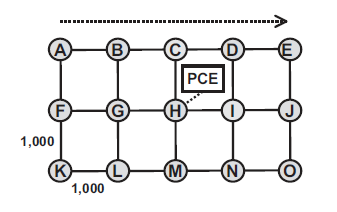
\includegraphics{Q1.PNG}
\end{figure}

\Q

%\item
Repeat Exercise 1, parts (a) and (b), except assume that a verification message
must be received by the source node indicating that the path has been
properly configured.
%\item

\Q

Repeat Exercise 1, parts (a) and (b), except assume that the grid topology
shown in the figure holds only for the data plane. Assume that the control plane
has a different topology such that the propagation delay between any two nodes
or between a node and the PCE is 20 \% longer than in the data plane.
%\item 

\Q

Consider a GMPLS-based implementation for establishing the AE demand
shown in Exercise 1. Consider two scenarios, one where pipelining of the
Resv message is not permitted, and one where it is permitted. Assume that a
path setup verification message is not required before transmission can begin.
\begin{enumerate}[label=\alph*-]
\item
If the switches at each node can be configured in 10 ms, how much sooner
can the source begin transmission when pipelining is used?
\item
If Node C
requires 40 ms to configure its switch, instead of 10 ms, how much sooner can
the source begin transmission when pipelining is used?
\end{enumerate}
%\item

\Q

In the figure below, all vacant wavelengths in the links are denoted above them respectively. 
\begin{figure}[tbh!]
\centering
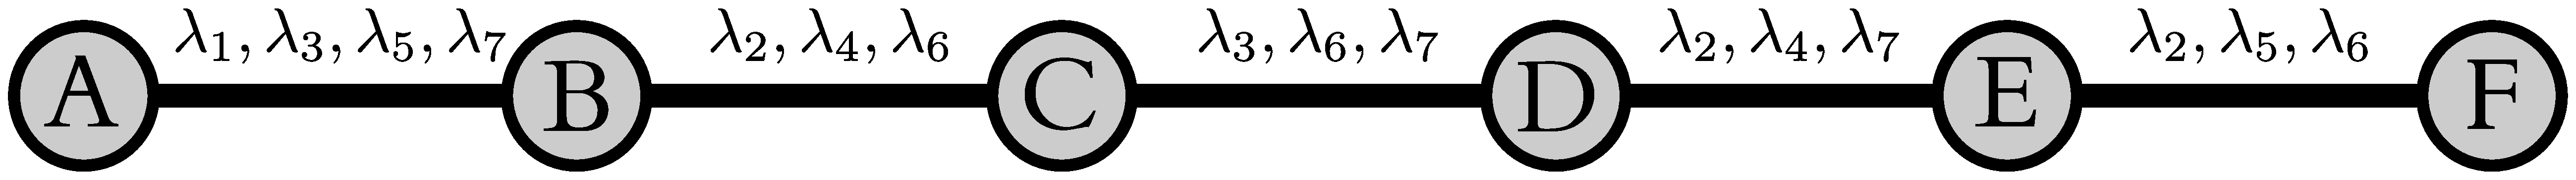
\includegraphics[scale=0.15]{lambda_bus.eps}
\label{fig:Q5}
\end{figure}

When node A wishes to initiate a connection to node F through nodes B to D, it advertises a path message to node B by considering the available wavelengths on its outgoing link (link AB). Each intermediate node takes in the path message of its previous node and establishes a new path message containing available wavelengths in both the previous node path message and its available outgoing link. If no such free wavelength can be found, the node drops whatever information and alerts that a regeneration must take place. Then it chooses as path mesage, the free wavelengths on its outgoing link, regardless of the path message of its previous node. Finally reaching to destination, a Resv message is delivered back in the opposite direction and initiated at destination node. The Resv message contains the chosen wavelength on links for establishing connections.

Answer the folowing questions:
\begin{enumerate}[label=\alph*-]
\item
Specify the path message and Resv message for all the links.
\item 
In which case or cases, does node E send a failure message back to the source? (you are free to consider wavelengths on EF arbitrarily)  
\end{enumerate}
%\item




%\end{enumerate}
\end{document}


